%-------------------------------------------------------------------------------
%                            BAB II
%               TINJAUAN PUSTAKA DAN DASAR TEORI
%-------------------------------------------------------------------------------
\fancyhf{} 
\fancyfoot[R]{\thepage}
\chapter{TINJAUAN PUSTAKA}

\par Untuk mendukung penelitian ini, maka dalam bab ini akan dikemukakan beberapa rumusan teori pendukung yang dikutip dari berbagai referensi baik dalam bentuk buku, artikel, maupun tulisan karya ilmiah lainnya termasuk hasil penelitian sebelumnya yang ada kaitannya dengan penelitian yang dilakukan.
\section{Landasan Teori}
%\subsection{System Usability Scale (SUS)}	
%\par \textit{System Usability Scale} (SUS) dikembangkan oleh \citep{brooke1996} sebagai sebuah pengukuran usability yang \textit{quick and dirty}. SUS menggunakan survei yang terdiri dari 10 pertanyaan, masing-masing memiliki 5 poin Likert sebagai tanggapan, output dari SUS berupa skor yang tampak mudah dipahami, dengan \textit{range} dari 0 hingga 100. Semakin besar skor berarti semakin baik \textit{usability}-nya. 

% \par Pengujian ini memerlukan kuesioner sebagai teknik pengumpulan informasi pengujian yang didapat dari responden mengenai aplikasi. Kuesioner terdiri dari 10 pertanyaan yang terdiri dari pertanyaan positif dan negatif. Pertanyaan positif terdapat pada nomor ganjil (1, 3, 5, 7, 9) dan pertanyaan negatif terdapat pada nomor genap (2, 4, 6, 8, 10). Setiap pertanyaan diberi bobot antara 0 - 4. Pertanyaan ganjil skor dihitung dengan cara bobot tiap pertanyaan (x\textsubscript{i}) dikurangi 1 (ditulis dengan x\textsubscript{i} - 1). Sedangkan pertanyaan genap skor dihitung dengan cara 5 dikurangi bobot tiap pertanyaan (x\textsubscript{i}) (ditulis dengan 5 - x\textsubscript{i}) \citep{ardiansyah2016}.

%-----------------------------------------------------------------------------%

% Baris ini digunakan untuk membantu dalam melakukan sitasi
% Karena diapit dengan comment, maka baris ini akan diabaikan
% oleh compiler LaTeX.

\section{Arsitektur FaceNet}
\par \textit{FaceNet} merupakan \textit{Convolutional Neural Network} (CNN) yang digunakan untuk pengenalan wajah, dikembangkan oleh peneliti dari Google dan dikenalkan pada tahun 2015 \citep{jose2019}. \textit{FaceNet} digunakan untuk mengekstraksi fitur dari gambar wajah seseorang. \textit{FaceNet} mengekstrak wajah menjadi vektor menggunakan \textit{deep} CNN. Vektor nilai atau \textit{vector embedding} yang dihasilkan dapat memetakan kemiripan wajah yang memiliki kedekatan posisi pada \textit{embedding space} \citep{rajagede2021}.

% Menambahkan gambar 
\begin{figure}[H]
\centering
\frame{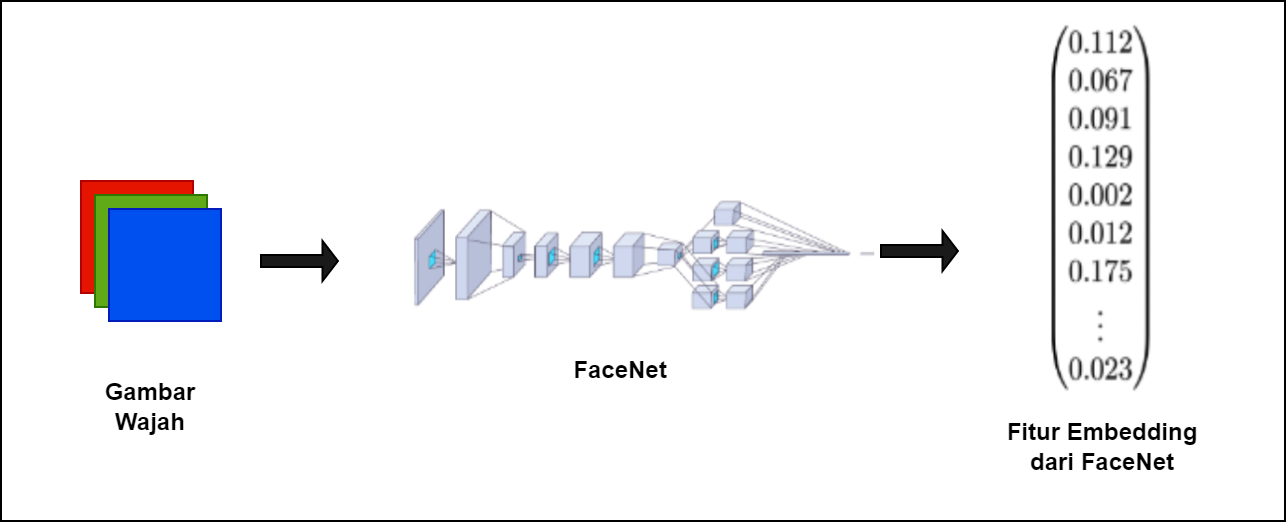
\includegraphics [width = 14cm, height= 5cm]{image/diagram_facenet}}
\caption{\textit{Desain} Arsitektur \textit{FaceNet}}.
\label{dig_facenet}
\end{figure}

\begin{figure}[H]
\centering
\frame{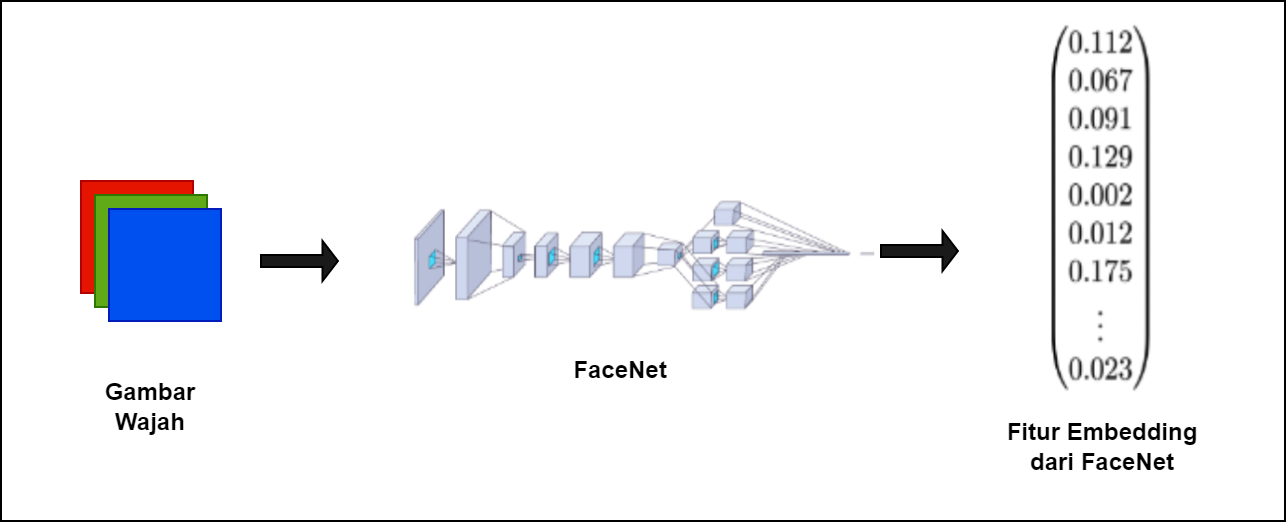
\includegraphics [width = 14cm, height= 5cm]{image/diagram_facenet}}
\caption{\textit{Desain} Arsitektur \textit{FaceNet}}.
\label{dig_facenet}
\end{figure}

\fancyhf{} 
\fancyfoot[R]{\thepage}

\begin{comment}
\bibliography{daftar-pustaka}
\end{comment}
